\section{Marco Metodológico y Snapping}

\begin{frame}{Marco Metodológico: Algoritmo de Snapping Lógico}
  \begin{columns}[T]
    \begin{column}{0.55\textwidth}
      \begin{itemize}
        \item \textbf{Problema:} La conversión directa de GeoJSON genera 
            "inflación topológica" (>49,000 nodos) por trazos no alineados.
        \item \textbf{Snapping Lógico (KDTree):} Proceso de anclaje automático 
            de trazos a estaciones en un radio de 50m.
        \item \textbf{Resultados:}
        \begin{itemize}
            \item Eliminación de "nodos fantasma".
            \item Reducción del \textbf{90\%} en la complejidad del grafo.
            \item Grafo final: 11,115 nodos operativos.
        \end{itemize}
      \end{itemize}
    \end{column}
    \begin{column}{0.40\textwidth}
      \begin{figure}
        \centering
        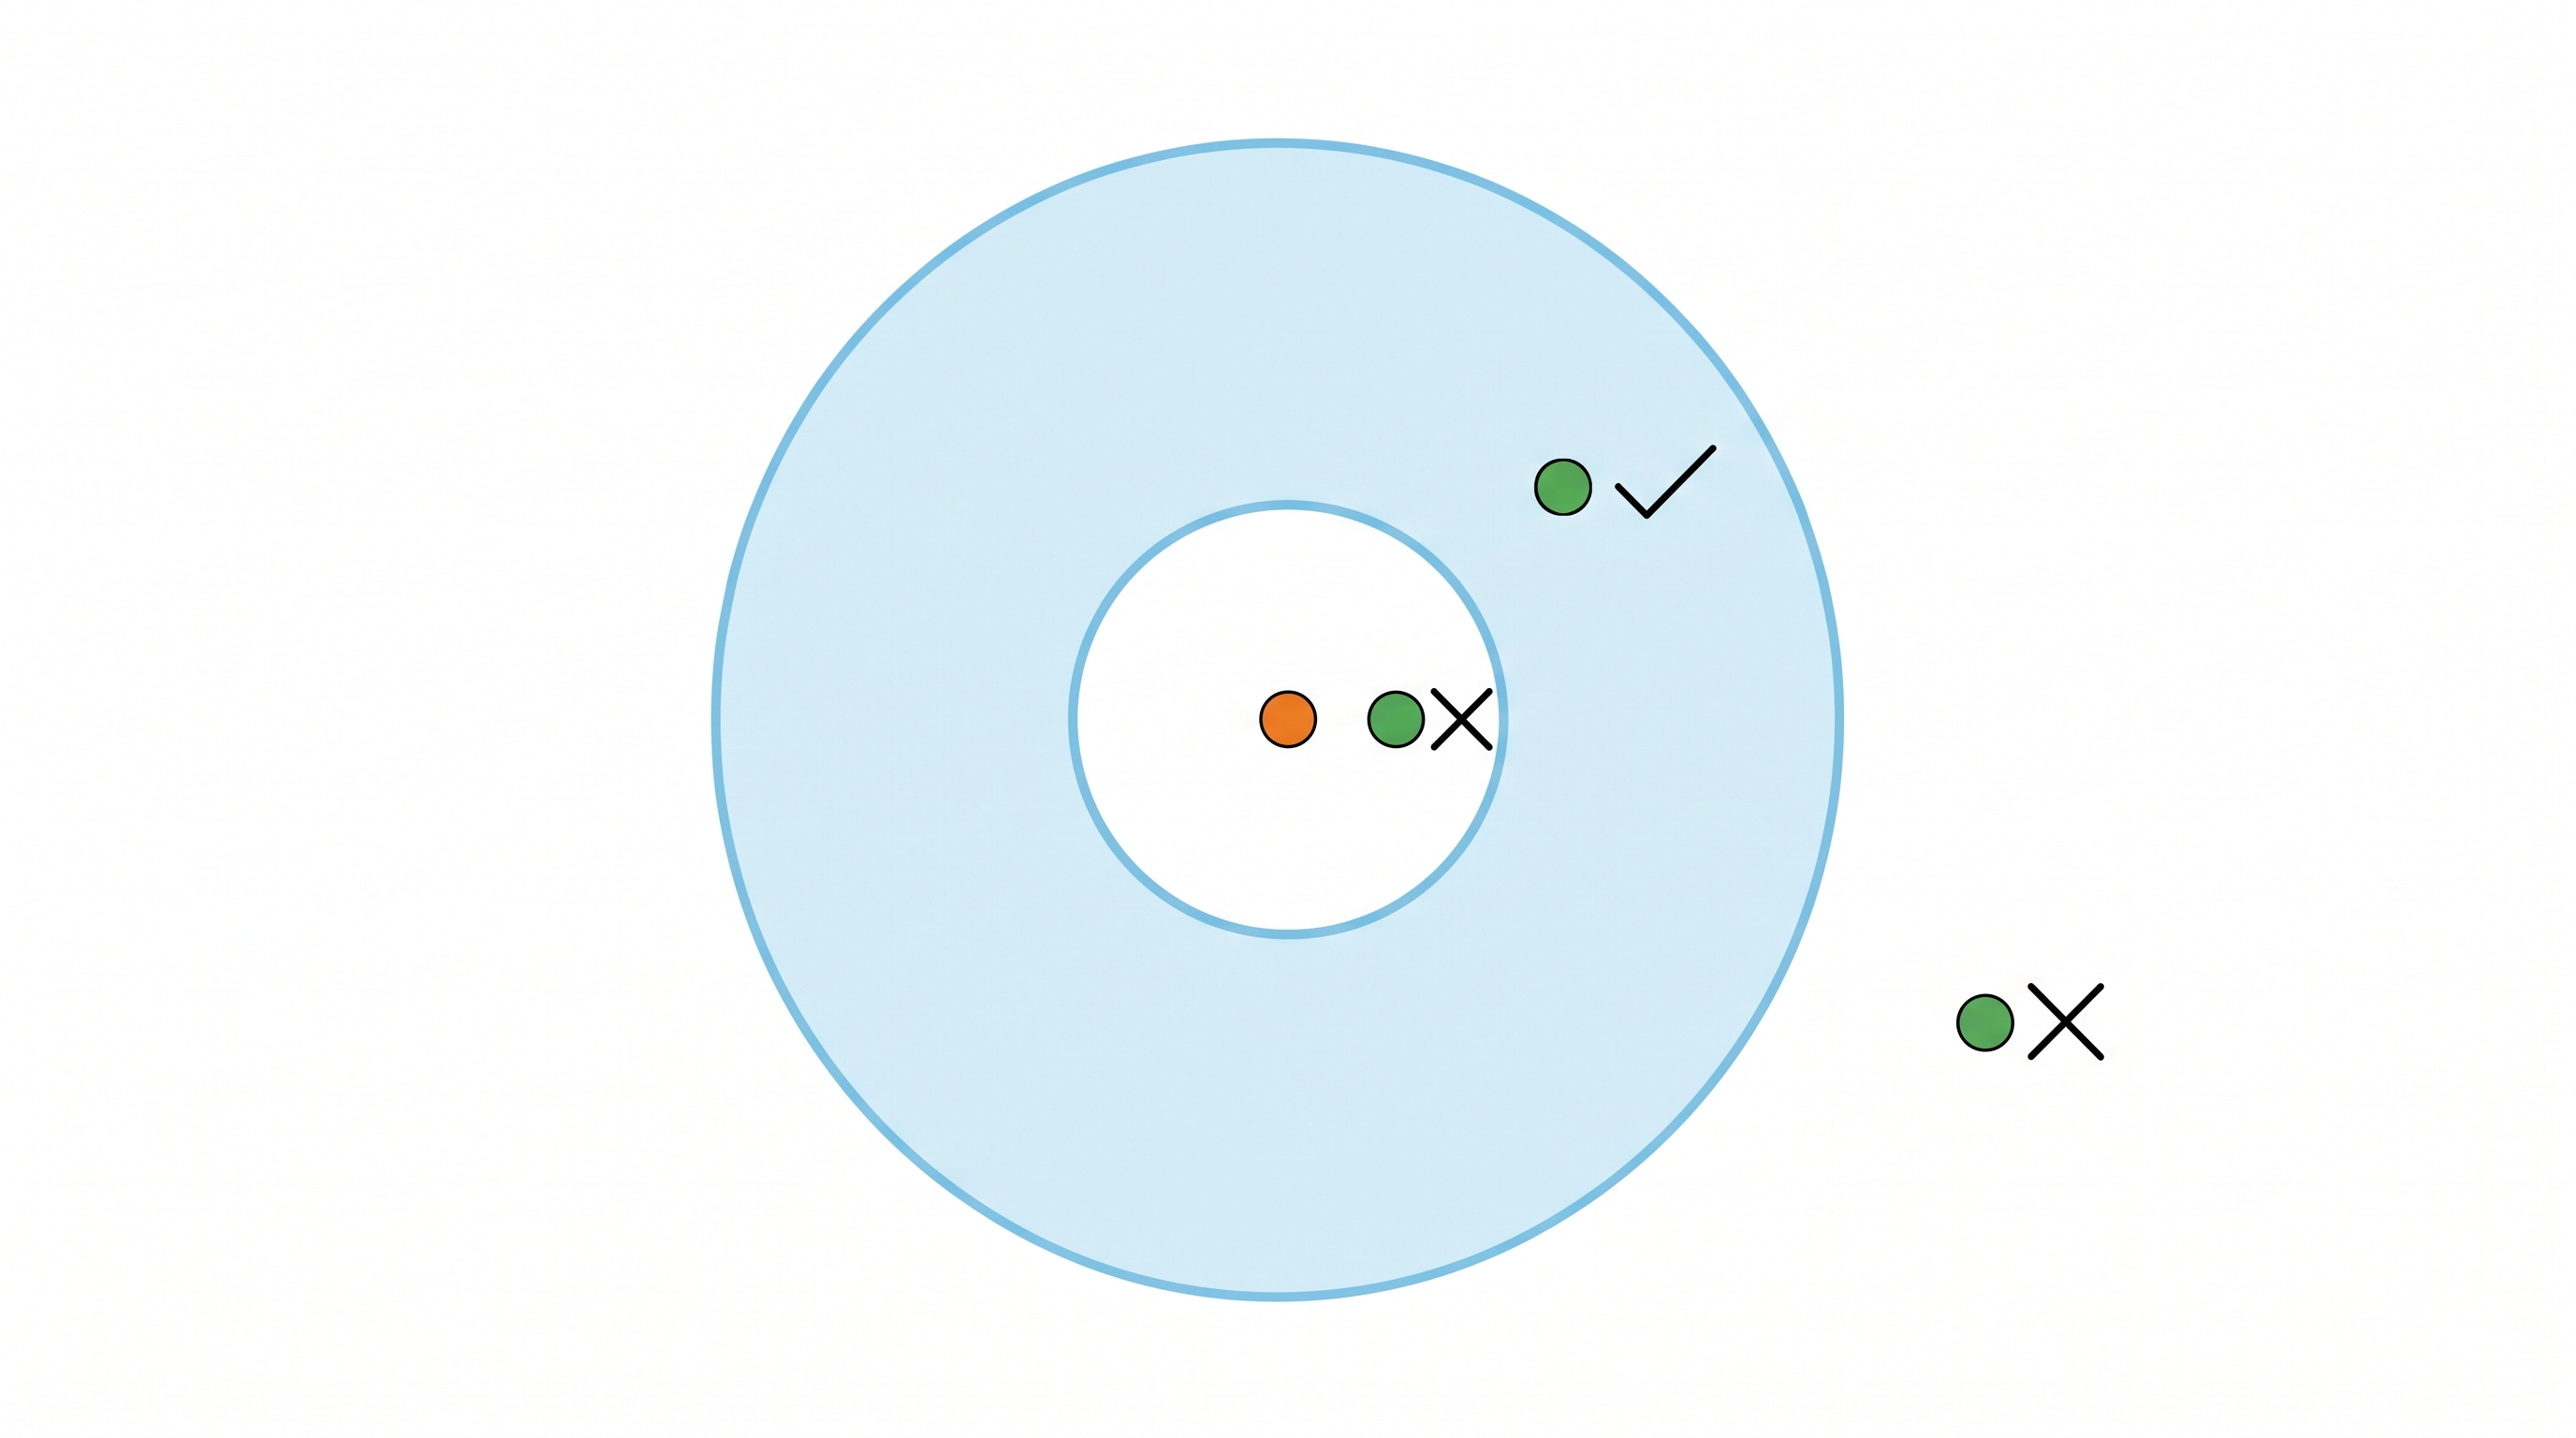
\includegraphics[width=0.8\textwidth]{img/F2Snapping.png}
        \caption{\tiny Radio de tolerancia y anclaje \cite{garibaldi2023vft}.}
      \end{figure}
    \end{column}
  \end{columns}
\end{frame}

% ========== DIAPOSITIVA 1: INDICADORES BASE ==========
\begin{frame}{Motor VFT: Jerarquía de Indicadores (F1 y F2)}
  \begin{columns}[c]
    % --- COLUMNA IZQUIERDA: ECUACIONES F1 Y F2 ---
    \begin{column}{0.50\textwidth}
      \small
      \textbf{F1: Espaciales y Cobertura}
      \begin{itemize}
          \item Cobertura: $C = \frac{A_{\text{cubierta}}}{A_{\text{total}}} \times 100$
          \item Fuerza Nodal: $FC_i = k_{\text{in}}(i) + k_{\text{out}}(i)$
      \end{itemize}
      
      \vspace{0.3cm}
      
      \textbf{F2: Eficiencia y Forma}
      \begin{itemize}
          \item Ruta Directa: $DI = \frac{d_{\text{red}}}{d_{\text{euclidiana}}}$
          \item Penalización: $W_{s,h} = T_{\text{walk}} + T_{\text{wait}}$
      \end{itemize}
    \end{column}
    
    % --- COLUMNA DERECHA: IMAGEN PANEL 1 ---
    \begin{column}{0.46\textwidth}
      \begin{figure}
        \centering
        
\includegraphics[width=\textwidth, height=0.65\textheight, keepaspectratio]{grafica_infraestructura.png}
        \caption{\tiny Panel 1: Infraestructura base.}
      \end{figure}
    \end{column}
  \end{columns}
  
  \vspace{0.2cm}
  \tiny \textcolor{gray}{Fuentes: \cite{garibaldi2023vft}.}
\end{frame}


% ========== DIAPOSITIVA 2: INDICADORES AVANZADOS ==========
\begin{frame}{Motor VFT: Jerarquía de Indicadores (F3 y F4)}
  \begin{columns}[c]
    % --- COLUMNA IZQUIERDA: ECUACIONES F3 Y F4 ---
    \begin{column}{0.50\textwidth}
      \small
      \textbf{F3: Topología y Rigor}
      \begin{itemize}
          \item Tiempo Viaje: $T = \frac{1}{N(N-1)} \sum t_{ij}$
          \item Intermediación: $B(v) = \sum \frac{\sigma_{st}(v)}{\sigma_{st}}$
      \end{itemize}
      
      \vspace{0.3cm}
      
      \textbf{F4: Vulnerabilidad}
      \begin{itemize}
          \item Robustez: $\Delta E = \frac{E_0 - E_f}{E_0}$
      \end{itemize}
    \end{column}
    
    % --- COLUMNA DERECHA: IMAGEN PANEL 2 ---
    \begin{column}{0.46\textwidth}
      \begin{figure}
        \centering
        
\includegraphics[width=\textwidth, height=0.65\textheight, keepaspectratio]{RedConectividad.png}
        \caption{\tiny Panel 2: Red de conectividad pura \cite{garibaldi2023vft}.}
      \end{figure}
    \end{column}
  \end{columns}
  
  \vspace{0.2cm}
  \tiny \textcolor{gray}{Fuentes: \cite{garibaldi2023vft}.}
\end{frame}
